% Created by tikzDevice version 0.12.6 on 2026-07-31 11:12:43
% !TEX encoding = UTF-8 Unicode
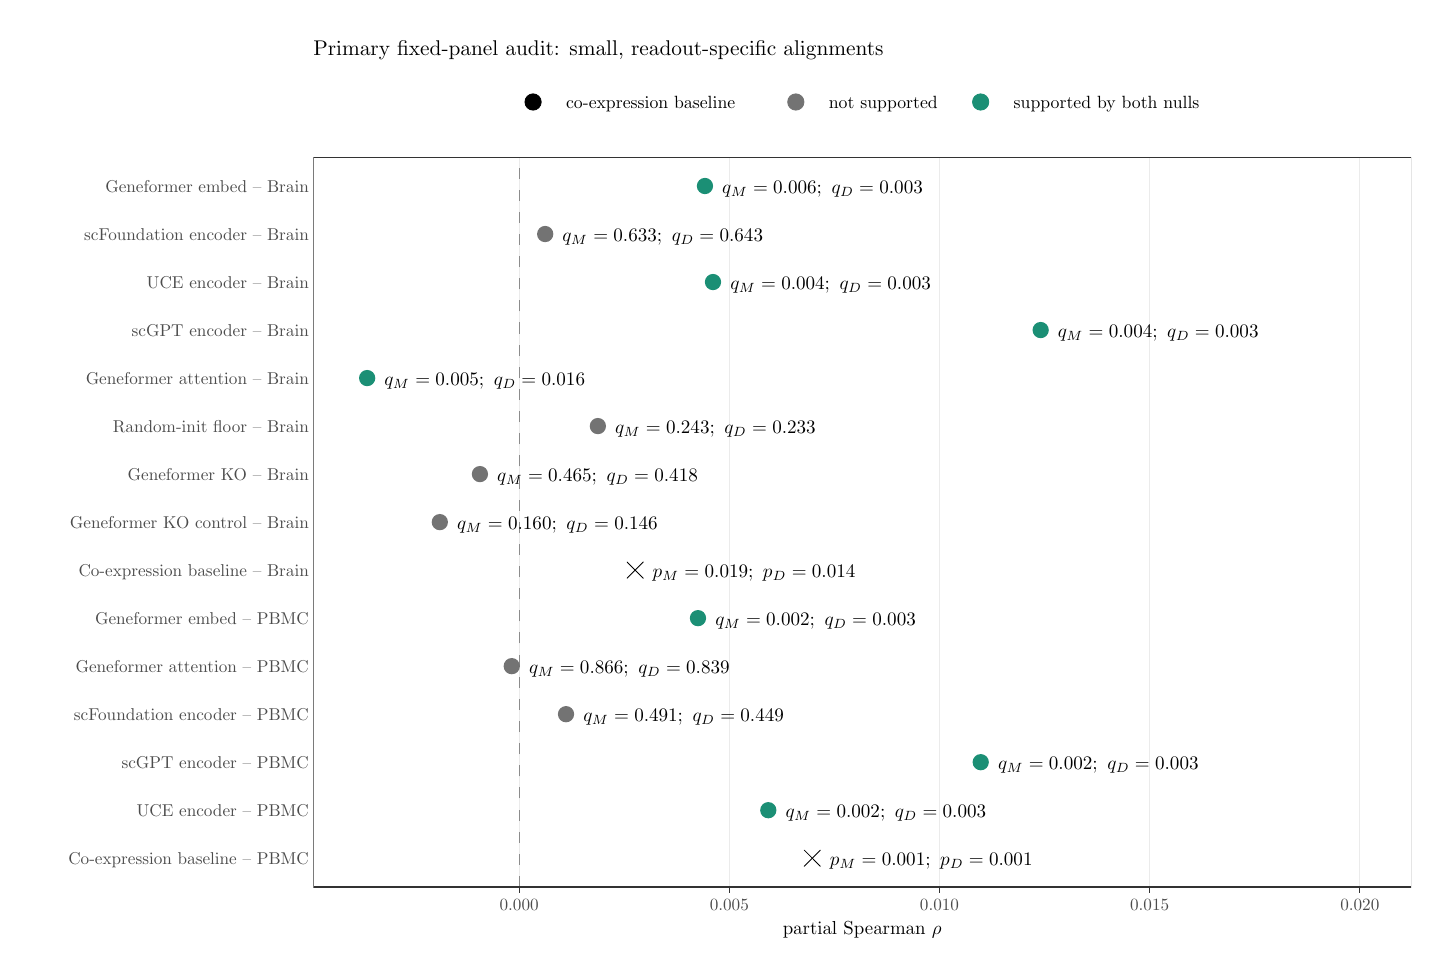
\begin{tikzpicture}[x=1pt,y=1pt]
\definecolor{fillColor}{RGB}{255,255,255}
\path[use as bounding box,fill=fillColor,fill opacity=0.00] (0,0) rectangle (505.89,332.44);
\begin{scope}
\path[clip] (  0.00,  0.00) rectangle (505.89,332.44);
\definecolor{drawColor}{RGB}{255,255,255}
\definecolor{fillColor}{RGB}{255,255,255}

\path[draw=drawColor,line width= 0.4pt,line join=round,line cap=round,fill=fillColor] (  0.00,  0.00) rectangle (505.89,332.44);
\end{scope}
\begin{scope}
\path[clip] (103.20, 21.91) rectangle (499.89,285.63);
\definecolor{fillColor}{RGB}{255,255,255}

\path[fill=fillColor] (103.20, 21.91) rectangle (499.89,285.63);
\definecolor{drawColor}{gray}{0.92}

\path[draw=drawColor,line width= 0.4pt,line join=round] (177.60, 21.91) --
	(177.60,285.63);

\path[draw=drawColor,line width= 0.4pt,line join=round] (253.54, 21.91) --
	(253.54,285.63);

\path[draw=drawColor,line width= 0.4pt,line join=round] (329.48, 21.91) --
	(329.48,285.63);

\path[draw=drawColor,line width= 0.4pt,line join=round] (405.42, 21.91) --
	(405.42,285.63);

\path[draw=drawColor,line width= 0.4pt,line join=round] (481.37, 21.91) --
	(481.37,285.63);
\definecolor{drawColor}{gray}{0.55}

\path[draw=drawColor,line width= 0.4pt,dash pattern=on 4pt off 4pt ,line join=round] (177.60, 21.91) -- (177.60,285.63);
\definecolor{fillColor}{RGB}{27,143,117}

\path[fill=fillColor] (244.73,275.22) circle (  2.94);
\definecolor{fillColor}{gray}{0.45}

\path[fill=fillColor] (187.00,257.87) circle (  2.94);
\definecolor{fillColor}{RGB}{27,143,117}

\path[fill=fillColor] (247.64,240.52) circle (  2.94);

\path[fill=fillColor] (366.04,223.17) circle (  2.94);

\path[fill=fillColor] (122.67,205.82) circle (  2.94);
\definecolor{fillColor}{gray}{0.45}

\path[fill=fillColor] (206.04,188.47) circle (  2.94);

\path[fill=fillColor] (163.42,171.12) circle (  2.94);

\path[fill=fillColor] (148.93,153.77) circle (  2.94);
\definecolor{drawColor}{RGB}{0,0,0}

\path[draw=drawColor,line width= 0.3pt,line join=round,line cap=round] (216.58,133.48) -- (222.45,139.36);

\path[draw=drawColor,line width= 0.3pt,line join=round,line cap=round] (216.58,139.36) -- (222.45,133.48);
\definecolor{fillColor}{RGB}{27,143,117}

\path[fill=fillColor] (242.21,119.07) circle (  2.94);
\definecolor{fillColor}{gray}{0.45}

\path[fill=fillColor] (174.92,101.72) circle (  2.94);

\path[fill=fillColor] (194.53, 84.37) circle (  2.94);
\definecolor{fillColor}{RGB}{27,143,117}

\path[fill=fillColor] (344.38, 67.02) circle (  2.94);

\path[fill=fillColor] (267.62, 49.67) circle (  2.94);

\path[draw=drawColor,line width= 0.3pt,line join=round,line cap=round] (280.59, 29.38) -- (286.46, 35.26);

\path[draw=drawColor,line width= 0.3pt,line join=round,line cap=round] (280.59, 35.26) -- (286.46, 29.38);

\node[text=drawColor,anchor=base west,inner sep=0pt, outer sep=0pt, scale=  0.69] at (250.98,272.55) {$q_M=0.006;\ q_D=0.003$};

\node[text=drawColor,anchor=base west,inner sep=0pt, outer sep=0pt, scale=  0.69] at (193.25,255.20) {$q_M=0.633;\ q_D=0.643$};

\node[text=drawColor,anchor=base west,inner sep=0pt, outer sep=0pt, scale=  0.69] at (253.90,237.85) {$q_M=0.004;\ q_D=0.003$};

\node[text=drawColor,anchor=base west,inner sep=0pt, outer sep=0pt, scale=  0.69] at (372.29,220.50) {$q_M=0.004;\ q_D=0.003$};

\node[text=drawColor,anchor=base west,inner sep=0pt, outer sep=0pt, scale=  0.69] at (128.93,203.15) {$q_M=0.005;\ q_D=0.016$};

\node[text=drawColor,anchor=base west,inner sep=0pt, outer sep=0pt, scale=  0.69] at (212.29,185.80) {$q_M=0.243;\ q_D=0.233$};

\node[text=drawColor,anchor=base west,inner sep=0pt, outer sep=0pt, scale=  0.69] at (169.68,168.45) {$q_M=0.465;\ q_D=0.418$};

\node[text=drawColor,anchor=base west,inner sep=0pt, outer sep=0pt, scale=  0.69] at (155.19,151.10) {$q_M=0.160;\ q_D=0.146$};

\node[text=drawColor,anchor=base west,inner sep=0pt, outer sep=0pt, scale=  0.69] at (225.83,133.75) {$p_M=0.019;\ p_D=0.014$};

\node[text=drawColor,anchor=base west,inner sep=0pt, outer sep=0pt, scale=  0.69] at (248.46,116.40) {$q_M=0.002;\ q_D=0.003$};

\node[text=drawColor,anchor=base west,inner sep=0pt, outer sep=0pt, scale=  0.69] at (181.17, 99.05) {$q_M=0.866;\ q_D=0.839$};

\node[text=drawColor,anchor=base west,inner sep=0pt, outer sep=0pt, scale=  0.69] at (200.78, 81.70) {$q_M=0.491;\ q_D=0.449$};

\node[text=drawColor,anchor=base west,inner sep=0pt, outer sep=0pt, scale=  0.69] at (350.63, 64.35) {$q_M=0.002;\ q_D=0.003$};

\node[text=drawColor,anchor=base west,inner sep=0pt, outer sep=0pt, scale=  0.69] at (273.87, 47.00) {$q_M=0.002;\ q_D=0.003$};

\node[text=drawColor,anchor=base west,inner sep=0pt, outer sep=0pt, scale=  0.69] at (289.85, 29.65) {$p_M=0.001;\ p_D=0.001$};
\definecolor{drawColor}{gray}{0.20}

\path[draw=drawColor,line width= 0.4pt,line join=round,line cap=round] (103.20, 21.91) rectangle (499.89,285.63);
\end{scope}
\begin{scope}
\path[clip] (  0.00,  0.00) rectangle (505.89,332.44);
\definecolor{drawColor}{gray}{0.30}

\node[text=drawColor,anchor=base east,inner sep=0pt, outer sep=0pt, scale=  0.62] at (101.60, 29.91) {Co-expression baseline -- PBMC};

\node[text=drawColor,anchor=base east,inner sep=0pt, outer sep=0pt, scale=  0.62] at (101.60, 47.26) {UCE encoder -- PBMC};

\node[text=drawColor,anchor=base east,inner sep=0pt, outer sep=0pt, scale=  0.62] at (101.60, 64.61) {scGPT encoder -- PBMC};

\node[text=drawColor,anchor=base east,inner sep=0pt, outer sep=0pt, scale=  0.62] at (101.60, 81.96) {scFoundation encoder -- PBMC};

\node[text=drawColor,anchor=base east,inner sep=0pt, outer sep=0pt, scale=  0.62] at (101.60, 99.31) {Geneformer attention -- PBMC};

\node[text=drawColor,anchor=base east,inner sep=0pt, outer sep=0pt, scale=  0.62] at (101.60,116.66) {Geneformer embed -- PBMC};

\node[text=drawColor,anchor=base east,inner sep=0pt, outer sep=0pt, scale=  0.62] at (101.60,134.01) {Co-expression baseline -- Brain};

\node[text=drawColor,anchor=base east,inner sep=0pt, outer sep=0pt, scale=  0.62] at (101.60,151.36) {Geneformer KO control -- Brain};

\node[text=drawColor,anchor=base east,inner sep=0pt, outer sep=0pt, scale=  0.62] at (101.60,168.71) {Geneformer KO -- Brain};

\node[text=drawColor,anchor=base east,inner sep=0pt, outer sep=0pt, scale=  0.62] at (101.60,186.06) {Random-init floor -- Brain};

\node[text=drawColor,anchor=base east,inner sep=0pt, outer sep=0pt, scale=  0.62] at (101.60,203.41) {Geneformer attention -- Brain};

\node[text=drawColor,anchor=base east,inner sep=0pt, outer sep=0pt, scale=  0.62] at (101.60,220.76) {scGPT encoder -- Brain};

\node[text=drawColor,anchor=base east,inner sep=0pt, outer sep=0pt, scale=  0.62] at (101.60,238.11) {UCE encoder -- Brain};

\node[text=drawColor,anchor=base east,inner sep=0pt, outer sep=0pt, scale=  0.62] at (101.60,255.46) {scFoundation encoder -- Brain};

\node[text=drawColor,anchor=base east,inner sep=0pt, outer sep=0pt, scale=  0.62] at (101.60,272.81) {Geneformer embed -- Brain};
\end{scope}
\begin{scope}
\path[clip] (  0.00,  0.00) rectangle (505.89,332.44);
\definecolor{drawColor}{gray}{0.20}

\path[draw=drawColor,line width= 0.4pt,line join=round] (177.60, 19.91) --
	(177.60, 21.91);

\path[draw=drawColor,line width= 0.4pt,line join=round] (253.54, 19.91) --
	(253.54, 21.91);

\path[draw=drawColor,line width= 0.4pt,line join=round] (329.48, 19.91) --
	(329.48, 21.91);

\path[draw=drawColor,line width= 0.4pt,line join=round] (405.42, 19.91) --
	(405.42, 21.91);

\path[draw=drawColor,line width= 0.4pt,line join=round] (481.37, 19.91) --
	(481.37, 21.91);
\end{scope}
\begin{scope}
\path[clip] (  0.00,  0.00) rectangle (505.89,332.44);
\definecolor{drawColor}{gray}{0.30}

\node[text=drawColor,anchor=base,inner sep=0pt, outer sep=0pt, scale=  0.62] at (177.60, 13.49) {0.000};

\node[text=drawColor,anchor=base,inner sep=0pt, outer sep=0pt, scale=  0.62] at (253.54, 13.49) {0.005};

\node[text=drawColor,anchor=base,inner sep=0pt, outer sep=0pt, scale=  0.62] at (329.48, 13.49) {0.010};

\node[text=drawColor,anchor=base,inner sep=0pt, outer sep=0pt, scale=  0.62] at (405.42, 13.49) {0.015};

\node[text=drawColor,anchor=base,inner sep=0pt, outer sep=0pt, scale=  0.62] at (481.37, 13.49) {0.020};
\end{scope}
\begin{scope}
\path[clip] (  0.00,  0.00) rectangle (505.89,332.44);
\definecolor{drawColor}{RGB}{0,0,0}

\node[text=drawColor,anchor=base,inner sep=0pt, outer sep=0pt, scale=  0.68] at (301.55,  4.66) {partial Spearman $\rho$};
\end{scope}
\begin{scope}
\path[clip] (  0.00,  0.00) rectangle (505.89,332.44);
\definecolor{fillColor}{RGB}{255,255,255}

\path[fill=fillColor] (170.67,293.63) rectangle (432.43,317.53);
\end{scope}
\begin{scope}
\path[clip] (  0.00,  0.00) rectangle (505.89,332.44);
\definecolor{fillColor}{RGB}{255,255,255}

\path[fill=fillColor] (174.67,297.63) rectangle (190.57,313.53);
\definecolor{drawColor}{RGB}{0,0,0}
\definecolor{fillColor}{RGB}{0,0,0}

\path[draw=drawColor,line width= 0.3pt,line join=round,line cap=round,fill=fillColor] (182.62,305.58) circle (  2.94);
\end{scope}
\begin{scope}
\path[clip] (  0.00,  0.00) rectangle (505.89,332.44);
\definecolor{fillColor}{RGB}{255,255,255}

\path[fill=fillColor] (269.62,297.63) rectangle (285.52,313.53);
\definecolor{drawColor}{gray}{0.45}
\definecolor{fillColor}{gray}{0.45}

\path[draw=drawColor,line width= 0.3pt,line join=round,line cap=round,fill=fillColor] (277.57,305.58) circle (  2.94);
\end{scope}
\begin{scope}
\path[clip] (  0.00,  0.00) rectangle (505.89,332.44);
\definecolor{fillColor}{RGB}{255,255,255}

\path[fill=fillColor] (336.41,297.63) rectangle (352.31,313.53);
\definecolor{drawColor}{RGB}{27,143,117}
\definecolor{fillColor}{RGB}{27,143,117}

\path[draw=drawColor,line width= 0.3pt,line join=round,line cap=round,fill=fillColor] (344.36,305.58) circle (  2.94);
\end{scope}
\begin{scope}
\path[clip] (  0.00,  0.00) rectangle (505.89,332.44);
\definecolor{drawColor}{RGB}{0,0,0}

\node[text=drawColor,anchor=base west,inner sep=0pt, outer sep=0pt, scale=  0.64] at (194.57,303.10) {co-expression baseline};
\end{scope}
\begin{scope}
\path[clip] (  0.00,  0.00) rectangle (505.89,332.44);
\definecolor{drawColor}{RGB}{0,0,0}

\node[text=drawColor,anchor=base west,inner sep=0pt, outer sep=0pt, scale=  0.64] at (289.52,303.10) {not supported};
\end{scope}
\begin{scope}
\path[clip] (  0.00,  0.00) rectangle (505.89,332.44);
\definecolor{drawColor}{RGB}{0,0,0}

\node[text=drawColor,anchor=base west,inner sep=0pt, outer sep=0pt, scale=  0.64] at (356.31,303.10) {supported by both nulls};
\end{scope}
\begin{scope}
\path[clip] (  0.00,  0.00) rectangle (505.89,332.44);
\definecolor{drawColor}{RGB}{0,0,0}

\node[text=drawColor,anchor=base west,inner sep=0pt, outer sep=0pt, scale=  0.77] at (103.20,322.41) {Primary fixed-panel audit: small, readout-specific alignments};
\end{scope}
\end{tikzpicture}
